\section{Methods}

\subsection{Dataset}
We use the melanoma segmentation dataset as published in the 2018 Lesion Boundary Segmentation Challenge by the International Skin Imaging Collaboration (ISIC) \citep{isic-2018-segmentation}. The dataset comprises dermatoscopic images with their corresponding ground truth segmentation masks \citep{ensambles-2016-codella}.

\par
The \emph{lesion} images were acquired by different dermatoscope types from several institutions, taken from all anatomic sites and from a historical sample of patients presented for skin cancer screening. Every image contains exactly one primary lesion. The distribution of disease states represent a modified "real world" setting (over-representation of malignancies) containing more benign lesions than malignant. All lesion images are named using the scheme ISIC\_\textless{image}\_id\textgreater{.jpg} with the \textless{image}\_id\textgreater{} being a 7-digit identifier \citep{isic-2018-segmentation}.

\par
The ground truth is represented by binary segmentation masks which indicate the location of the primary skin lesion within each input image. Mask images follow a similar naming scheme, namely  ISIC\_\textless{image\_id}\textgreater{\_segmentation.png}, and have the exact same dimensions as the lesion images. The masks are represented by a single-channel 8-bit continuous region, where each pixel is either 0 (background - area outside of the primary lesion) or 255 (foreground - area inside the primary lesion). The ground truth images were obtained using several techniques (e.g. fully automated algorithm; manual polygon tracing by human expert annotators), but all data were reviewed by practicing dermatologists with expertise in dermoscopy \citep{isic-2018-segmentation,ensambles-2016-codella}.

\par
The dataset is divided into train, validation and test sets with 2’594, 100 and 1’000 images respectively. The train and validation datasets contain the exact same number of ground truth segmentation mask images whereas the test dataset does not. The test dataset is used for the final evaluation of the challenge submission and hence does not contain any segmentation masks. Figure \ref{datasets} shows image size distribution per dataset.

\begin{figure}[ht]
\centering
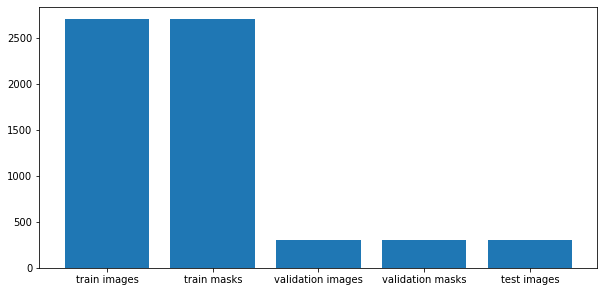
\includegraphics[width=\columnwidth]{assets/datasets.png}
\caption[Datasets]
{Image distribution in the train, validation and test datasets (ISIC 2018 segmentation challenge).}
\label{datasets}
\end{figure}

The images in each dataset show a spectrum of variations in terms of quality (e.g. sharpness, lighting conditions, coloring etc.) and added noise (e.g. hair, rulers, bubbles etc.). Furthermore, the resolution of the images varies significantly. The train dataset has 206 different dimensions, ranging from a resolution of 540 x 722 pixels to 4499 x 6748 pixels. The validation dataset has 21 different resolutions, ranging from 480 x 640 pixels to 4461x 6641 pixels. Lastly, the test dataset has 114 different resolutions, ranging from 480 x 640 pixels to 4519 x 6808 pixels. Figure \ref{lesion_images} shows three examples of lesion images and their corresponding binary segmentation masks.

\begin{figure}[ht]
\centering
\includegraphics[width=\columnwidth]{assets/lesion_images.pdf}
\caption[Lesion Images]
{Three different images with different noise on the top with their corresponding binary masks at the bottoms.}
\label{lesion_images}
\end{figure}


% \begin{itemize}
%   \item Define your task in a clear, concise manner
%   \item Formally describe each model under investigation. Include your baseline and experimental models at minimum.
%   \item For each model, describe its infrastructure and assumptions (if applicable).
% \end{itemize}
